% Chapter 2

\chapter{Selective Alignment} % Main chapter title

\label{selective_alignment} % For referencing the chapter elsewhere, use \ref{Chapter2} 

%----------------------------------------------------------------------------------------

\section{Background}
\label{sec:background}

Since its introduction in 2008~\citep{lister,nagalakshmi,mortazavi2008mapping}, transcriptome
profiling via RNA-seq has become a popular and widely-used technique to profile gene-
and transcript-level expression, and to identify and assemble novel transcripts.
Expression estimation is often done with the goal of subsequently performing
differential expression analysis on the gene abundance profiles. In response to
improvements in RNA-seq quality and read lengths, as well as significant
improvements in the available quantification methods, it has also become
increasingly common to perform quantification and differential testing at the
transcript level. Recently, very
fast computational methods~\citep{sailfish,kallisto,salmon,fleximer} for
transcript abundance estimation have been developed which obtain their speed, in part, by forgoing
the traditional step of aligning the reads to the reference genome
or transcriptome. These methods have gained popularity due to their markedly
smaller computational requirements and their simplicity of use compared to more
traditional quantification ``pipelines'' that require alignment of the
sequencing reads to the genome or transcriptome, followed by the subsequent
processing of the resulting BAM file to obtain quantification estimates.

In various assessments on simulated data~\citep{kanitz2015comparative,germain2016rnaonthebench,zhang2017evaluation}, these lightweight 
methods have compared favorably to well-tested but much slower methods for
abundance estimation, like RSEM~\citep{li2011rsem}, coupled with alignment methods such
as Bowtie2~\citep{bowtie2}. However, assessments based primarily (or entirely)
upon simulated data often fail to capture important aspects of real experiments,
and similar performance among methods on such simulated datasets does not
necessarily generalize to experimental data. Popular methods for transcript
quantification~\citep{rnaskim,fleximer,salmon,kallisto,sailfish,li2011rsem,heraem,hensman2015fast,glaus2012identifying}
differ in many aspects, ranging from how they handle read mapping and alignment,
to the optimization algorithms they employ, to differences in their
generative models or which biases they attempt to model and correct. These differences
are often obscured when analyzing simulated data, since aspects of experimental
data that can lead to substantial divergence in quantification estimates are not
always properly recapitulated in simulations.

We focus on the effect of read
mapping on the resulting transcript quantification estimates. To compare the
effect of different alignment and mapping methods on RNA-seq transcript
quantification and related downstream analysis, we have picked tools from three
different categories of mapping strategies: (1) unspliced alignment of RNA-seq reads
directly to the transcriptome, (2) spliced alignment of RNA-seq reads to the
annotated genome (with subsequent projection to the transcriptome), and
(3) (unspliced) lightweight mapping (\qm) of RNA-seq reads directly to the
transcriptome. While numerous different lightweight mapping approaches
exist~\citep{sailfish,rnaskim,kallisto,rapmap,fleximer}, and the degree to which
they diverge from alignment-based methods can differ, a key feature shared by
such approaches is that they do not validate predicted fragment mappings via an
alignment score, which precludes them from discerning loci where the best
mappings would not admit a reasonable-scoring alignment (i.e.\@ spurious
mappings). Furthermore, the focus on speed means that such methods tend not to
explore sub-optimal mapping loci, despite the fact that such loci might admit
the best alignment scores and therefore be the most likely origin for a
fragment. We show that differences in how reads are aligned or mapped can lead
to considerable differences in the predicted abundances. Specifically, we find
that lightweight mapping approaches, %\citep{sailfish,kallisto,rapmap,fleximer} ,
which are generally highly concordant with traditional alignment approaches in
simulated data, can lead to quite different abundance estimates from
alignment-based methods in experimental data. These differences happen across a
large number of samples, but the magnitude of the differences can vary
substantially from sample to sample. We also find that these differences appear
even when exactly the same optimization procedure is used to infer transcript
abundances.  Instead, these differences are a result of the different mapping and alignment
approaches returning distinct, and sometimes even disjoint, mapping loci for
certain reads.

Due to the absence of a ground truth in experimental data, it is 
difficult to categorically specify which approaches produce more accurate estimates.
However, by investigating the divergence we observe
among the quantifications produced by different methods, and the differences
in read mapping that lead to this divergence in quantifications, we uncover
some primary failure cases of different alignment and mapping strategies. This
leads us to compare and combine the results of different alignment strategies,
and allows us to curate a set of oracle alignments for experimental samples.
  Comparing various approaches to the oracle provides further evidence for a
  hypothesis, raised in~\citet{selaln} and ~\citet{heraem}, that lightweight
  mapping approaches may suffer from spurious mappings leading to a decrease in
  the resulting quantification accuracy compared to alignment-based approaches.
  We also demonstrate that, even among alignment-based approaches, non-trivial
  differences arise between quantifications based upon mapping to the
  transcriptome (using Bowtie2~\citep{bowtie2}) and quantifications based upon
  mapping to the genome and subsequently projecting these alignments into
  transcriptomic coordinates (using STAR~\citep{star}). Both of these
  alignment-based approaches sometimes disagree with the oracle, but do so for
  different subsets of fragments and to a varying degree among different
  samples. 
  

Finally, we introduce an improved mapping algorithm, selective alignment (\hsa),
that is designed to remain fast, while simultaneously eliminating many of the
mapping errors made by lightweight approaches. \hsa is integrated into the \salmon~\citep{salmon}
transcript quantification tool. Our proposed method increases
both the sensitivity and specificity of fast read mapping. It relies upon
alignment scoring to help differentiate between mapping loci that would
otherwise be indistinguishable due to, for example, similar exact matches along
the reference. Our approach also determines when even the best mapping for a
read exhibits insufficient evidence that the read truly originated from the
locus in question, allowing it to avoid spurious mappings. 
We also attempt to address one of the failure modes of direct alignment against
  the transcriptome, compared to spliced alignment to the genome: when a sequenced fragment originates
  from an unannotated genomic locus bearing sequence-similarity to an annotated
  transcript, it can be falsely mapped to the annotated transcript since the
  relevant genomic sequence is not available to the method. We describe a procedure
  that makes use of MashMap~\citep{jain2018fast} to identify and extract such
  sequence-similar \emph{decoy} regions from the genome. The normal \salmon
  index is then augmented with these decoy sequences, which are handled in a
  special manner during mapping and alignment scoring, leading to a reduction in
  such cases of false mappings. We benchmark two variants of this approach; one in which
we extract a small collection of decoy sequences via the procedure mentioned
above (designated as \texttt{SA}), and one in which we align against the
transcriptome and whole genome simultaneously, allowing us to detect fragments
that better map to a non-transcriptomic target.  The latter approach, which 
essentially treats the whole genome as \emph{decoy} sequence, is denoted as 
\texttt{SAF}. We benchmark these approaches on both simulated data and a broad collection of
experimental RNA-seq samples, and demonstrate that they lead to improved
concordance with the abundance estimates obtained via quantification
following traditional alignment.


\section{Materials and Methods}
\subsection{Selective alignment}
\label{subsec:meth_sa}

Selective alignment is based on the pufferfish indexing data structure first
described in~\citep{pufferfish}. Moreover, the index is augmented with the
relevant decoy sequence (either restricted decoy sequence as described
in~\Cref{subsec:meth_decoy} or the entire genome) which is marked during
indexing and handled in a special manner during alignment scoring.


The mapping approach works in 5 distinct phases (for paired-end reads).
First, exact matches between the read and transcriptome are collected.
Second, the set of transcripts to be considered for further processing are
extracted. Third, exact match chaining and chain scoring, using the algorithm
of~\citet{minimap2}, is used to determine the relevant putative mapping loci
for the read. Fourth (for paired-end reads), the mappings for the first and
second read of the pair are matched to determine the mapping loci for the
whole fragment. Finally, the computed mapping loci are scored using extension
alignment scoring~\citep{minimap2,suzuki2018introducing} before, after and 
between the exact matches belonging to the highest-scoring chain for each 
mapping. In this final step, information about the decoy sequences is used to
determine which mappings are considered valid and which are not (details are
provided below).

In the first phase of the mapping algorithm, uni-MEMs~\citep{debga} are
collected between the sequenced fragment (with each read end treated
separately) and the index. The uni-MEMs are found via k-mer lookup, and then
are extended maximally until the end of a unitig is encountered, the
end of the read is encountered, or a mismatch is encountered.  If uni-MEM 
extension terminates because it reaches the end of a unitig or because of a 
mismatch, search advances in the read and subsequent k-mers are queried in 
the index to collect other uni-MEMs shared between the read and the index.
This process is repeated until the end of the read, and results in a collection 
of uni-MEMs --- matches between the read and the index that can be efficiently 
decoded into the implied matches between the read and the reference.

In the second phase, uni-MEMs are projected to their corresponded reference
loci, and the exact matches are collated by reference and orientation. Let
$M$ denote the number of matches for the transcript, orientation pair with
the maximum number of matches for the current read. An optional
(user-determined) filtering policy is applied, whereby any transcript and
orientation pair that does not have at least $\tau M$ matches is
discarded from further consideration. The value of $\tau$ is a user-specified
fraction, set as $0.65$ by default.  This optional filtering policy, termed 
as ``filtering before chaining'', is disabled by default, but can be enabled 
via the command-line option \texttt{--hitFilterPolicy BEFORE}. Note that it
was not enabled in our experiments and the default was used. 

Next, matches along each transcript, orientation pair are sorted and
compacted. This compaction is necessary since it is possible to have matches
that are directly adjacent on both the read and reference, but which were not
extracted as a single exact match during the first phase because the
underlying uni-MEM terminated. This compaction phase eliminates such
fragmentation due to uni-MEM termination, and reduces the number of exact
matches that must be considered by the chaining algorithm. Candidate mapping
locations are determined by applying the chaining algorithm of
minimap2~\citep{minimap2} to the exact matches for each transcript passing the
previous filter. If multiple equally-good positions for a read along a
transcript, in terms of their chaining score, are discovered, they are all
propagated downstream in the mapping procedure until mappings for paired-end
reads are merged. Likewise, if a read is determined to map to a transcript in
both the forward and reverse-complement orientation, then all equally-best
mapping loci in both orientations are propagated downstream in the mapping
procedure.  Let $S$ be the best chaining score obtained for any mapping of
the current read.  An optional filter is applied where any mapping with a 
chaining score less than $\tau' S$ is discarded from further consideration.
By default, this filter, termed as ``fitering after chaining'', is enabled 
by default and $\tau'$ is set as 0.65.

For paired-end reads, the pairs are merged by determining, for each
transcript, the locations of the read ends that respect the expected mapping
constraints (e.g. that the leftmost position of the reverse complement read
is to the right of the leftmost position of the forward-strand read, and the
distances between the reads is less than the maximum allowed insert size). If
passed the appropriate flag \texttt{--allowDovetails}, then
dovetailed~\citep{bt2manual} mappings are allowed, but they are prioritized
below any non-dovetailed mapping.


All putative mappings are scored using the ksw2~\citep{minimap2,suzuki2018introducing} library
for alignment extension. We note that we compute only the optimal alignment
score, and not the details of the alignment itself (i.e.\@ the CIGAR string),
which improves the speed of this mapping validation. To avoid redundant
computation of the same alignment problem (which is quite prevalent when mapping
directly to the transcriptome, as many alignments to alternatively-spliced
transcripts will be identical), \hsa maintains a per-read alignment cache. This
alignment cache is a hash table where the key is a hash of the reference
transcriptome substring where the read is predicted to align, and the value is
the previous alignment score computed for such a substring. Thus, if multiple
transcripts would produce identical alignments for the same read, because the
read maps to identical regions of these transcripts, \hsa is able to avoid
this redundant work.

Finally, all of the relevant alignments are grouped by their associated
alignments scores. Any alignments that fall below the (user-provided) threshold
(default of $0.65$ of the maximum obtainable alignment score) for a minimum
valid alignment score are discarded. During alignment scoring, the score of the
best alignment for a given fragment to any decoy sequence as well as to any
non-decoy sequence is computed and stored. If the best alignment score to a
decoy sequence is strictly greater than the best alignment score to a non-decoy
sequence, then all of the fragment's mappings are considered invalid and the
fragment is not considered for quantification. Otherwise, any alignments to
decoy sequences are filtered out, and the remaining alignments to valid
transcripts are further processed by \salmon using range-factorized equivalence
classes~\citep{ddfact}, which allows the relevant information about the scores
for the different alignments of the read to be appropriately summarized and used
for quantification.

\subsection{Analysis details}
\label{subsec:notes}

\paragraph{A note on the difference between \hsa and \saf}
This manuscript introduces the idea of selective alignment over a reference sequence 
indexed using the pufferfish~\citep{pufferfish} data structure, implemented in the \salmon program. The index
takes as input a set of decoy sequences, which are not part of the reference transcriptome 
and are, therefore, not quantified. In our analyses, we considered the performance of the selective alignment 
algorithm when paired with two different sets of decoys as input. In the first approach, referred to as \hsa in the manuscript, 
the index is built on the transcriptome and regions of the genome that
have high sequence similarity with the transcriptome. In the second approach, referred to as \saf, 
the complete genome is included in the pufferfish index as a set of decoys. Hence, the 
index for \hsa contains a smaller portion of the genome, whereas the \saf index contains
the full genome. Also, note that selective alignment replaces the \qm algorithm previously 
used in the \salmon program.

\paragraph{A note on on orphan and dovetail mappings}
We attempted to normalize for some mapping-related differences between
methods that have little to do with the ability of the aligner to appropriately
find the correct loci for a read, and instead have to do with constraints placed
on what constitutes a valid mapping. Specifically, when projecting to the
transcriptome, STAR disallows orphan mappings (cases where one end of a fragment
aligns to a transcript but the other end does not). Likewise it is recommended
practice in existing alignment-based quantification tools~\citep{rsem,hensman2015fast,glaus2012identifying},
when using Bowtie2, to discard discordant and orphaned alignments. Thus, in our
analyses, we disallowed orphaned mappings so that, in paired-end datasets, the
pair is discarded if only one end of a fragment is mapped, or if the fragment
ends only map to distinct transcripts. To be consistent with the default
behavior of Bowtie2, the configurations of \qm and \hsa were also set to disallow dovetailed mappings (mappings where the
first mapped base of the reverse complement strand read is upstream of the first
mapped base of the forward strand read). While Bowtie2's scoring function (when performing global alignment) 
does not allow insertions or deletions to occur at the beginning or end of the read, we attempted to minimize the 
effect of this structural constraint on alignments by setting the \texttt{--gbar} parameter to 1.

\paragraph{A note on genomic alignment, as used in this manuscript.}
We explored differences that arise between quantification
based on alignment of the sequencing reads to the genome and the transcriptome. 
We considered genomic alignment here to be the process of
alignment to the genome --- with the benefit of a known annotation ---
with subsequent projection to the transcriptome. That is, genomic
alignment is characterized based on running STAR (with appropriate parameters)
to align the reads to the genome, and then making use of the
transcriptomically-projected alignments output by STAR via the
\texttt{--quantMode TranscriptomeSAM} flag (as would be used in e.g.\@ a
STAR\citep{star}/RSEM\citep{rsem}-based quantification pipeline). Such an
approach is necessarily concerned only with how well STAR is able to align the
sequenced reads to the annotated transcriptome of the organism being
assayed, and our assessment is concerned only with the accuracy of
quantification of known and annotated isoforms. Importantly, spliced alignment of
RNA-seq reads to the genome can be a useful tool in tackling a broader range of
problems and in a larger set of cases than can unspliced alignment to a known
transcriptome. For example, spliced alignment of sequencing reads to the genome
can be done in the absence of an annotation of known isoforms, and can be used
to help identify novel exons, isoforms, or transcribed regions of the genome,
while unspliced alignment to a pre-specified set of transcripts does not admit
this type of analysis. Further, alignment directly to the genome can easily cope
with events like intron retention, which are more difficult to account for when
using methods that align reads to the transcriptome.

\paragraph{A note on the influence of short transcripts on quantification.} 
The human GENCODE v29 reference includes transcripts as short as 8bp, which is
much shorter than a single sequencing read or the typical fragment length in
most RNA-seq experiments. While RNA-seq might not be the appropriate method to
quantify these transcripts, depending on the alignment method, they may have
mapped reads and obtain non-zero expression values. In our analyses, we observed
that lightweight mapping methods that do not perform end-to-end alignment tend
to assign reads to shorter transcripts when there is an exact match. This effect
has been explored in some detail by~\citet{wu2018limitations}. In such a
scenario, it is hard to judge the true origin of the read, and while this may
lead to some differences between mapping and alignment-based methods, we showed that the
differences in quantification estimates for short transcripts account for only a
very small fraction of the overall differences between methods. 
Since it is difficult to judge how these shorter transcripts, and the
reads aligning to them, should be handled, we simply highlighted this issue and
refrained from suggesting a particular strategy or attempting to determine which
method performed better or worse on transcripts shorter than $300$bp. 

\section{Results}
\subsection{Comparison between alignment and mapping algorithms}
\label{subsec:overview}

For benchmarking, we used \qm and \hsa (with either the similar-sequence decoy regions or the whole genome), 
both available in the \salmon~\citep{salmon} program, where
\qm is a representative for lightweight mapping methods and \hsa is our proposed
method that performs sensitive lightweight mapping
followed by an efficient alignment-scoring procedure. For unspliced read
alignment directly to the transcriptome, we used Bowtie2~\citep{bowtie2}, which
is an accurate and popular tool for unspliced alignment. Similarly, we used
STAR~\citep{star} as representative of methods that perform spliced read
alignment against the genome. We chose STAR, in particular, since it has the
ability to project the aligned reads to transcriptomic coordinates, which allowed
us to use a consistent quantification method, and also because it is part of the
popular STAR~\citep{star}/RSEM~\citep{li2011rsem} transcript abundance estimation
pipeline.

We used \salmon as the main quantification engine in our analyses since it supports
quantification from \qm, \hsa, and via the output of traditional aligners. To
the best of our knowledge, \salmon is the only quantification tool
that has support for both lightweight mapping approaches and quantification
using traditional alignments. We used \salmon in alignment mode to process the
output from Bowtie2 and STAR. In tests on the initial simulated data, we also
included RSEM. To remove variability in the quantification methods that is
ancillary to our focus on mapping and alignment, we used the \texttt{--useEM}
flag in \salmon for comparison against the EM-based algorithm of RSEM. Likewise,
to eliminate variability due to the target set of transcripts being quantified,
we passed the \texttt{--keepDuplicates} option to \salmon when indexing for
subsequent mapping using quasi-mapping or \hsa\footnote{Though we performed
  indexing here with \texttt{--keepDuplicates} and quantification with
  \texttt{--useEM}, this is done only to eliminate controllable sources of
  variability between methods so as to isolate, as much as possible, the effect
  of differences in mapping. We generally recommend that duplicate transcripts
  are discarded during indexing, and that the offline phase of quantification is
  performed using the variational Bayesian EM.}.
  
Where mentioned, the ``strict'' and ``RSEM'' versions of Bowtie2 and STAR refer to these tools
being run with the flags recommended in the RSEM manual~\citep{rsem_manual},
which disallow insertions, deletions and soft-clipping in the resulting
alignments. The difference between them is that the ``strict'' versions are
quantified using \salmon and the ``RSEM'' versions using the RSEM expression
calculation method. Throughout the text, we refer to the pipelines by the
following shorthand (more details about the methods are given in~\Cref{subsec:notes}, and~\Cref{tab:methods} and
the full command line options provided to
each tool are given in~\Cref{subsec:commands}):

\begin{itemize}
\item Bowtie2 -- Alignment with Bowtie2 to the target transcriptome and allowing alignments with indels,
  followed by quantification using \salmon in alignment mode.

\item Bowtie2\_strict -- Alignment with Bowtie2 to the target transcriptome and disallowing alignments with indels (i.e.\@ using the same parameters as those used by RSEM), followed by quantification using \salmon in alignment mode.

\item Bowtie2\_RSEM -- Alignment with Bowtie2 to the target transcriptome and disallowing alignments with indels, followed by quantification using RSEM.

\item STAR -- Alignment with STAR to the target genome (aided with the GTF annotation of the transcriptome) and projected to the transcriptome allowing alignments with indels and soft clipping, followed by quantification using \salmon in alignment mode.

\item STAR\_strict -- Alignment with STAR to the target genome (aided with the GTF annotation of the transcriptome) and projected to the transcriptome and disallowing alignments with indels or soft clipping, followed by quantification using \salmon in alignment mode.

\item STAR\_RSEM -- Alignment with STAR to the target genome (aided with the GTF annotation of the transcriptome) and projected to the transcriptome and disallowing alignments with indels or soft clipping, followed by quantification using RSEM.

\item quasi -- quasi-mapping directly to the target transcriptome, coupled with quantification using \salmon in non-alignment mode.

\item SA -- Selective alignment directly to the target transcriptome and a set of decoy sequences (high similarity with the transcriptome), coupled with quantification using \salmon in non-alignment mode. (Details in~\Cref{subsec:meth_decoy} and~\Cref{subsec:meth_sa}.)

\item SAF -- Selective alignment (full) directly to the target transcriptome and the genome, treated as decoy sequences, coupled with quantification using \salmon in non-alignment mode. (Details in~\Cref{subsec:meth_sa}.)

\end{itemize}

\subsection{Performance on typical simulations}
\label{subsec:initial_sim}

We used a Polyester\citep{polyester}-simulated dataset to show the performance
of various methods on synthetic data. The distribution of transcript
expression for this simulation was learned from an experimental (human) sample
(\texttt{SRR1033204}, quantified using Bowtie2 with \salmon). We computed the
Spearman correlation of quantification estimates from all the pipelines when
compared against a known ground truth (in terms of read count). To simulate
technical variation, we ran each simulation 10 times using the same input
abundance distribution, but varying the random seed used by Polyester.

We observed that, though there are differences in correlation, all pipelines had
somewhat similar overall performance on this simulated dataset, with the
exception of STAR, which exhibited the lowest correlation. On this data, \qm
performed better than aligning to the genome (and then projecting to the
transcriptome) but marginally worse than doing traditional alignment
against the transcriptome (both with and without the strict parameters for
Bowtie2). We observed that \hsa performed better than aligning to
the transcriptome using Bowtie2, except when quantified using RSEM, though the
difference in this scenario is quite small. Finally, \saf performed very similarly
to \hsa in these simulations, though \hsa, using the smaller decoy set, performed marginally
better given that, in reality, all of the reads truly derive from annotated transcripts (with 
only very minor modifications due to simulated sequencing error).

Overall, the analysis on this synthetic dataset gives an impression that
quantifications resulting from the different mapping approaches exhibit similar
accuracy, and that all approaches quantify transcript abundances relatively
well. While this is true for these simulated data, we show below that this
observation does not generalize to experimental data. We posit that this is
because, though great advancements have been made in improving the realism of
simulated RNA-seq data, these simulations still fail to capture some of the
complexities of experimental data. We describe below one particular way in which
the realism of the simulated data can be increased by accounting for variations
between the sequenced reads and the transcriptome used for quantification.

\begin{table}[h!]
 \centering
 \begin{tabular}{cc}
   \hline
   Method & Truth \\
   \hline
Bowtie2 & $\numprint{0.9398301926562247} \pm \numprint{0.0005186918970326195}$ \\
Bowtie2\_strict & $\numprint{0.9405956345734323} \pm \numprint{0.0005809629124469005}$ \\
Bowtie2\_RSEM & $\numprint{0.9486443627046326} \pm \numprint{0.00041347255434347646}$ \\
SA & $\numprint{0.9449382937796003} \pm \numprint{0.0004501130954645799}$ \\
SAF & $\numprint{0.9439140545571167} \pm \numprint{0.00043373801948212254}$ \\
quasi & $\numprint{0.9374138292232805} \pm \numprint{0.000384870000382568}$ \\
STAR & $\numprint{0.9148946561265291} \pm \numprint{0.0005669491265107912}$ \\
STAR\_strict & $\numprint{0.9120259972984865} \pm \numprint{0.0005283357323574355}$ \\
STAR\_RSEM & $\numprint{0.9193216410605245} \pm \numprint{0.0003819284328874204}$ \\
 \hline
\end{tabular}
 \caption{\textbf{Spearman correlation against ground truth for data simulated using Polyester.} Note that the
 counts were based on a real sample from human.}
 \label{tab:swim}
\end{table}


\subsection{Performance on simulations from a variant mouse transcriptome}
\label{subsec:variant_sim}

An observation we made from the previous simulation was that disallowing
indels using the RSEM parameters (used for strict and RSEM versions) for Bowtie2 and STAR 
did not adversely affect accuracy compared to using the default parameters of each method.
We hypothesized that this is because the reads are simulated exactly from the
reference transcriptome that is being used for alignment and quantification, and
only sequencing errors (which are taken to consist entirely of substitution
errors) are introduced by the simulator. Yet, in experimental data,
the sample being quantified likely exhibits variation with respect to the
reference against which the reads are aligned. Some of these variants will be
single nucleotide polymorphisms (SNPs), while others will be indels and yet
others may be larger structural variants. Thus, restricting alignments to disallow
indels seems undesirable, unless one is quantifying
against a personalized reference that is known to contain the variants present
in the sample, which can potentially improve the accuracy of transcript
quantification~\citep{munger2014rna, makemickhappy}.

\begin{table}[h!]
 \centering
 \begin{tabular}{ccc}
   \hline
    Method & PWK & GRCm38.91\\
   \hline
	Bowtie2 & $\numprint{0.9390547489909096} \pm \numprint{0.0005423716560320824}$ & $\numprint{0.9342585400075698} \pm \numprint{0.0005502869415911537}$ \\
	Bowtie2\_strict & $\numprint{0.9391991582111261} \pm \numprint{0.0006183598098204462}$  & $\numprint{0.9225599199303829} \pm \numprint{0.0006781735587586356}$ \\
	Bowtie2\_RSEM & $\numprint{0.9415665798526123} \pm \numprint{0.0006230660996204234}$  & $\numprint{0.9246353350736198} \pm \numprint{0.0007076367571536213}$ \\
	SA & $\numprint{0.9405906153456616} \pm \numprint{0.0006146431086302259}$  & $\numprint{0.9361289848562275} \pm \numprint{0.000651158720069728}$ \\
	SAF & $\numprint{0.9393659086781574} \pm \numprint{0.0006260361972251335}$ & $\numprint{0.9345925078430021} \pm \numprint{0.0006115191901658021}$ \\
	quasi & $\numprint{0.9400522777457361} \pm \numprint{0.0005945130831824111}$  & $\numprint{0.9263377367507948} \pm \numprint{0.00045217051077881844}$ \\
	STAR & $\numprint{0.9346754134269342} \pm \numprint{0.0005011476978394499}$ & $\numprint{0.9293280761197311} \pm \numprint{0.0005925177293300123}$ \\
	STAR\_strict & $\numprint{0.9344104800680494} \pm \numprint{0.00048668643239887946}$  & $\numprint{0.9141531401179572} \pm \numprint{0.0006040301196884785}$ \\
	STAR\_RSEM & $\numprint{0.9365502350437739} \pm \numprint{0.0005599078377258275}$ & $\numprint{0.9159213041990121} \pm \numprint{0.0006500440156524715}$ \\
 \hline 
\end{tabular}
 \caption{\textbf{Spearman correlation against ground truth for data simulated using Polyester.} Note that the reads were simulated using the reference
 containing the mouse PWK strain's variants.}
 \label{tab:mouse}
\end{table}

To test the hypothesis that disallowing indels in the alignments will adversely
affect quantification accuracy when simulating from a reference transcriptome
containing realistic variants compared to the reference, we performed the
following experiment. We obtained VCF files from the Sanger Mouse Genomes
website\footnote{\url{ftp://ftp-mouse.sanger.ac.uk/REL-1410-SNPs_Indels/}}
describing the variants present in the PWK mouse strain. Using
g2gtools~\citep{g2gtools}, we generated a copy of the GRCm38.91 transcriptome containing
the variants (including indels) present in the PWK strain and simulated reads
from this transcriptome. The results presented in the first column
of~\Cref{tab:mouse} show that when reads are aligned against the PWK strain's
reference and indels are disallowed, the quantification estimates are as
accurate as those derived from alignments allowing indels, as expected. However, when we aligned the
reads back to the original mouse reference transcriptome (version GRCm38.91), we
observed that, indeed, Bowtie2 performed better than Bowtie2\_strict (second column
of~\Cref{tab:mouse}), and that, generally, disallowing indels in alignments has
a negative effect on quantification accuracy.

To further analyze the influence of indels on quantification, we aligned the
transcript sequences from the PWK strain and the original reference using
edlib~\citep{vsovsic2017edlib} and counted the total length of indels in each
transcript compared to the unaltered transcript's original length (we refer to
this quantity as the indel ratio). We then sorted the transcripts in descending
order by their indel ratios, and evaluated at each cumulative subset, the
difference in correlation with the truth between the quantifications using the
alignment method and its ``strict'' variant. We evaluated this quantity
increasing the cumulative subsets by 1000 transcripts at each step. We observed
that the difference between methods is highest in transcripts that have a larger
indel ratio (\Cref{fig:indelcorr}). Hence, the impact of disallowing indels in
the alignment can be considerable for reads that originate from transcripts that
differ from the reference due to the presence of indels, and this can eventually lead
to such transcripts being substantially misquantified.

\begin{figure}[t!]
    \centering
    \begin{subfigure}[t]{0.45\textwidth}
        \centering
	    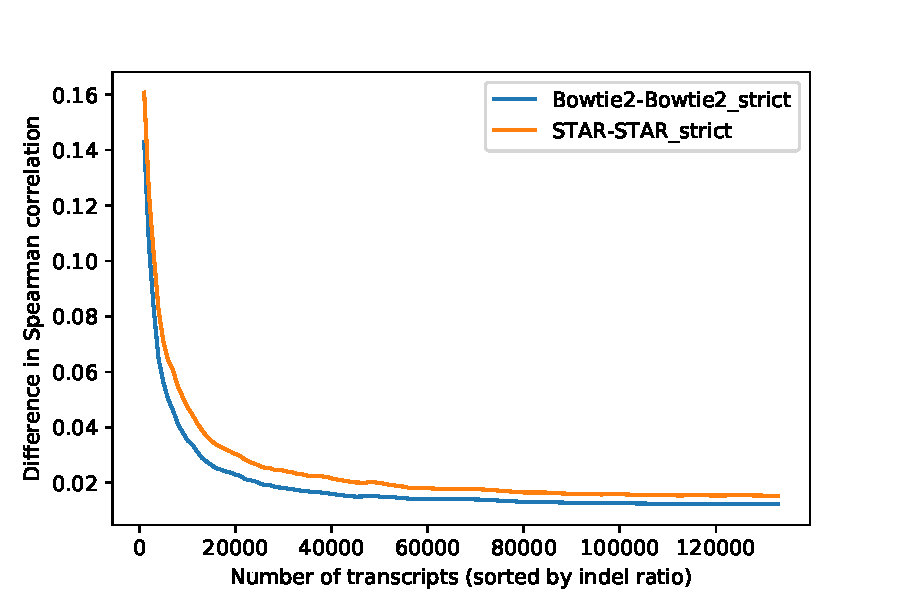
\includegraphics[width=\linewidth]{selal/full_indel.pdf}
      \caption{\label{subfig:indel_strat_full}}
    \end{subfigure}
    ~
    \begin{subfigure}[t]{0.45\textwidth}
        \centering
	    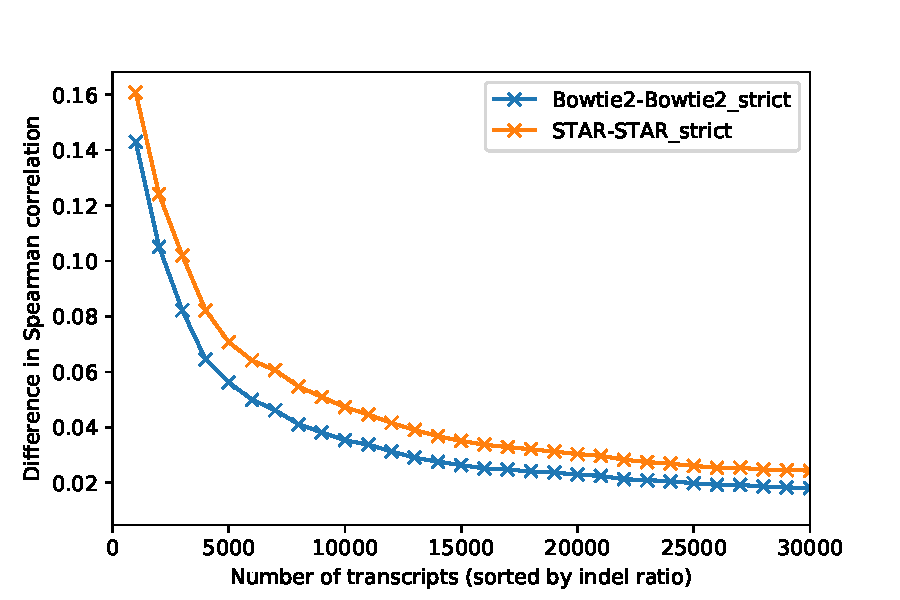
\includegraphics[width=\linewidth]{selal/zoomed_indel.pdf}
      \caption{\label{subfig:indel_strat_zoomed}}
    \end{subfigure}
    \caption{\textbf{Impact on quantification accuracy when disallowing indels.} (a) Difference in correlation with the truth between both alignment
      methods and their ``strict'' variants, where indels are disallowed, on all mouse transcripts sorted by their indel ratios. (b) The same plot restricted
      to the $30,000$ transcripts with the largest indel ratio.}
    \label{fig:indelcorr}
\end{figure}

Due to both the theoretical concerns and the practical evidence shown here, we
proceeded in representing the alignment-based methods by using Bowtie2 and STAR in
our comparisons, only in configurations that allow indels to occur in the
alignments, and excluded from our analyses the ``strict'' and ``RSEM'' versions of the pipelines. 

\subsection{Randomly sampled experiments from NCBI database}
\label{subsec:experimental}

It is crucial to evaluate the performance of the various tools on data from real
experiments, that can be vastly more complex than even state-of-the-art simulations
and can include processes, both known and unknown, that affect the underlying
data in complicated ways. To analyze the accuracy of existing tools and study
the impact of the artifacts (like the above) on experimental datasets, we
randomly selected 200 human RNA-seq experiments from the NCBI database
for further investigation. We then filtered the selected samples to include
only paired-end libraries having a minimum read length of 75bp. After applying
these filters, we were left with a set of $109$ samples (69 bulk and 40 full-length single-cell). Before further
processing, we applied adapter and (light) quality trimming using TrimGalore~\citep{trimgalore, cutadapt}\footnote{The effect of trimming on the overall results was
relatively minimal (result not shown).}. We also observed that the overall mapping
rates across samples tended to be similar between all methods
(\Cref{fig:mrate}), though Bowtie2 tends to exhibit the highest sensitivity
(i.e.\@ aligns the most reads) on average.
Subsequently, we quantified all $109$ samples using each of the remaining pipelines.

\begin{figure}[t!]
    \centering
     \begin{subfigure}[t]{0.7\textwidth}
     \centering
  	  	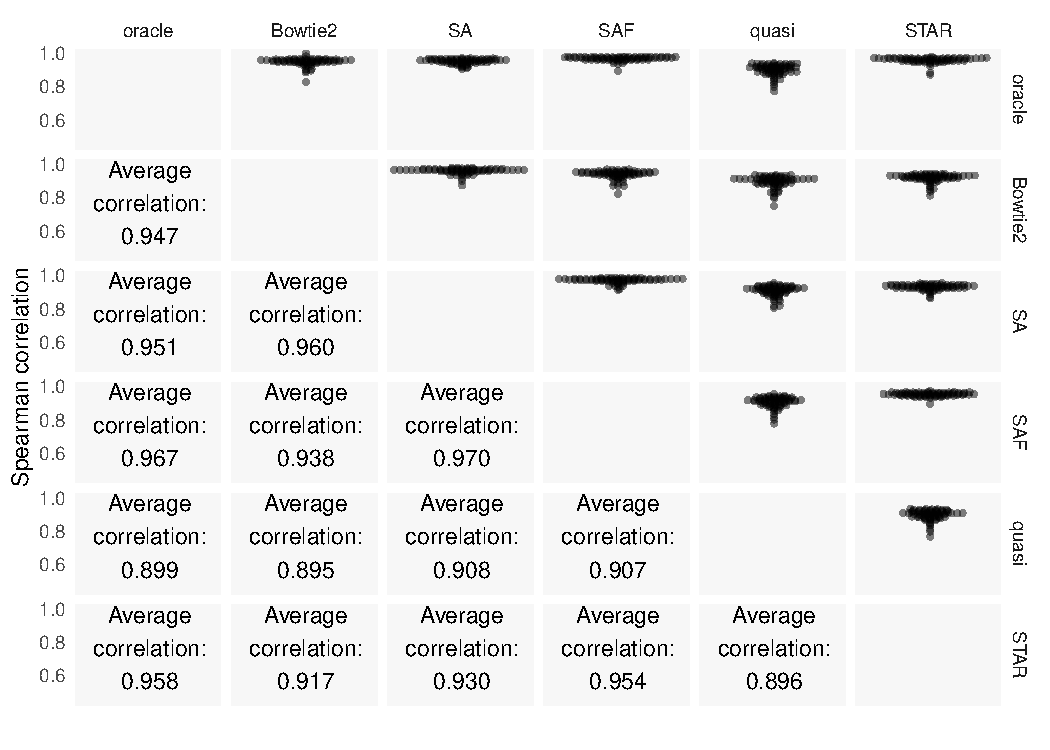
\includegraphics[width=\linewidth]{selal/bulk_pairwise_correlations_real_data.pdf}
		\caption{Bulk}
    \end{subfigure}
     \begin{subfigure}[t]{0.7\textwidth}
     \centering
  	  	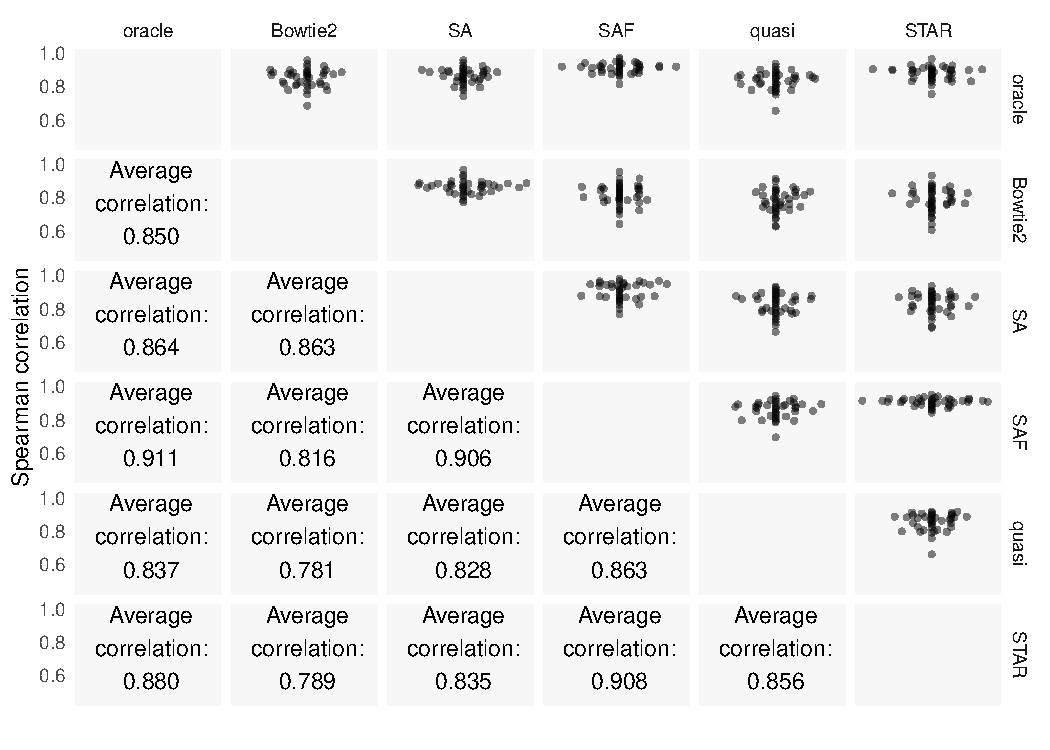
\includegraphics[width=\linewidth]{selal/singlecell_pairwise_correlations_real_data.pdf}
		\caption{Single-cell}
    \end{subfigure}     
     \caption{\textbf{Performance of each method on real bulk and single-cell datasets.} 
      The top half of the matrix shows swarm plots of the pairwise correlations of the TPM values predicted by different
       approaches on the experimental samples. The bottom half shows the average
       Spearman correlation across the $109$ bulk and single-cell samples.}
    \label{fig:swarm}
\end{figure}


Since no ground truth transcript abundances were available for these $109$
experimental datasets, it became more difficult to analyze the accuracy of the
different pipelines. However, we explored, manually, some of
  the cases where differences in mappings and alignments led to divergence of quantification
  estimates between methods. Between Bowtie2, \qm, and STAR, the mappings seemed to fall
  into one of two major categories. In one case, Bowtie2 seemed to be appropriately
  reporting a more comprehensive set of best-scoring mappings than STAR and \qm.
  In the other case, the resulting sequencing fragment seemed to clearly arise from some unannotated
  region of the genome --- either from intronic or intergenic sequence --- and it was
  spuriously assigned by Bowtie2 and \qm to some set of annotated transcripts (though not
  always the same set).  This led to the following observation: when the fragment truly originates 
  from the annotated transcriptome, Bowtie2 appears the most sensitive and accurate method in aligning the read to
  the appropriate subset of transcripts, as is also supported by the variant transcriptome
  simulations from~\Cref{subsec:variant_sim}. However, this same sensitivity can
  sometimes lead Bowtie2 to spuriously align reads to the annotated
  transcriptome when they are better explained by some other (unannotated)
  genomic locus. In this latter case, STAR tends to report the correct alignment
  for the read, and, appropriately refrains from reporting alignments to
  annotated transcripts. These complications, in which reads are sequenced from
  underlying fragments that either overlap or are sequence-similar to annotated
  transcripts, is yet another factor that leads to divergent behavior between
  different mapping and alignment approaches, but which is not commonly
  considered in simulation.

These observations led us to combine information from both
  Bowtie2 and STAR to derive an \emph{oracle} method, that avoids the obvious
  shortcomings, as listed above, of either of the constituent methods. To derive
  the oracle alignments in each sample, we used the following approach. First, we
  aligned the reads for the sample using both Bowtie2 and STAR, and for STAR we
  retained both the genomic and transcriptomic BAM files (i.e.\@ we considered all of
  the alignments that STAR was able to produce to the genome, as well as those
  that it was able to successfully project to the transcriptome). Subsequently,
  we examined the reads that were aligned to the transcriptome using Bowtie2, and
  were aligned to the genome using STAR, but which STAR did not project to the
  transcriptome. For each such read, we examined the best-scoring transcriptomic
  alignment records produced by Bowtie2 as well as the best-scoring genomic
  alignment records produced by STAR. We compared the quality of these alignments
  between the tools by first parsing the extended CIGAR string (the \texttt{MD}
  tag), and assigning a score to each reported alignment. In our
  scoring scheme, we assigned 1 to every matched base while penalizing soft-clips,
  SNPs and indels by assigning a score of 0. We reported the score of an alignment
  as the sum of the number of properly matched bases along the ends of the read.
  If the transcriptomic alignment of Bowtie2 was of equal or higher quality to
  the genomic alignment, then we retained the transcriptomic alignment. Otherwise,
  we marked the fragment's alignment records for removal. We then processed the
  original Bowtie2 BAM file for the sample, removing alignments for all
  fragments that have been marked for removal. The result was a filtered version
  of the Bowtie2 BAM file in which spurious transcriptomic alignments have been
  removed. We quantified the sample by providing \salmon with this filtered BAM
  file, and refer to the resulting quantification estimates as the
  \emph{oracle} estimates for this sample.

While other complex alignment scenarios may occur, these oracle
  estimates represent quantification based on the set of alignments that avoid
  the obvious shortcomings of the different approaches being considered.
  Specifically, being based on alignment rather than lightweight-mapping, all
  alignments benefit from the improved sensitivity of Bowtie2's search procedure
  and are guaranteed to support a matching of the read to the reference of at
  least the required quality. Further, since these alignments are derived from
  Bowtie2, they likely correspond to a correct and comprehensive set of
  transcripts when the fragment does, in fact, originate from the annotated
  transcriptome. Finally, in the case where the fragment does not originate from
  an annotated transcript, and is instead the product of transcription from an
  unannotated locus, novel splicing, or intron retention, the corresponding
  alignment records have been removed using information from STAR's alignment 
  to the genome, so that the fragment is not spuriously
  allocated to annotated transcripts. Thus, we treated the oracle quantifications
  as a proxy for the true abundances in the experimental samples.

\begin{figure}[t!]
    \centering
    \begin{subfigure}[t]{0.45\textwidth}
        \centering
	    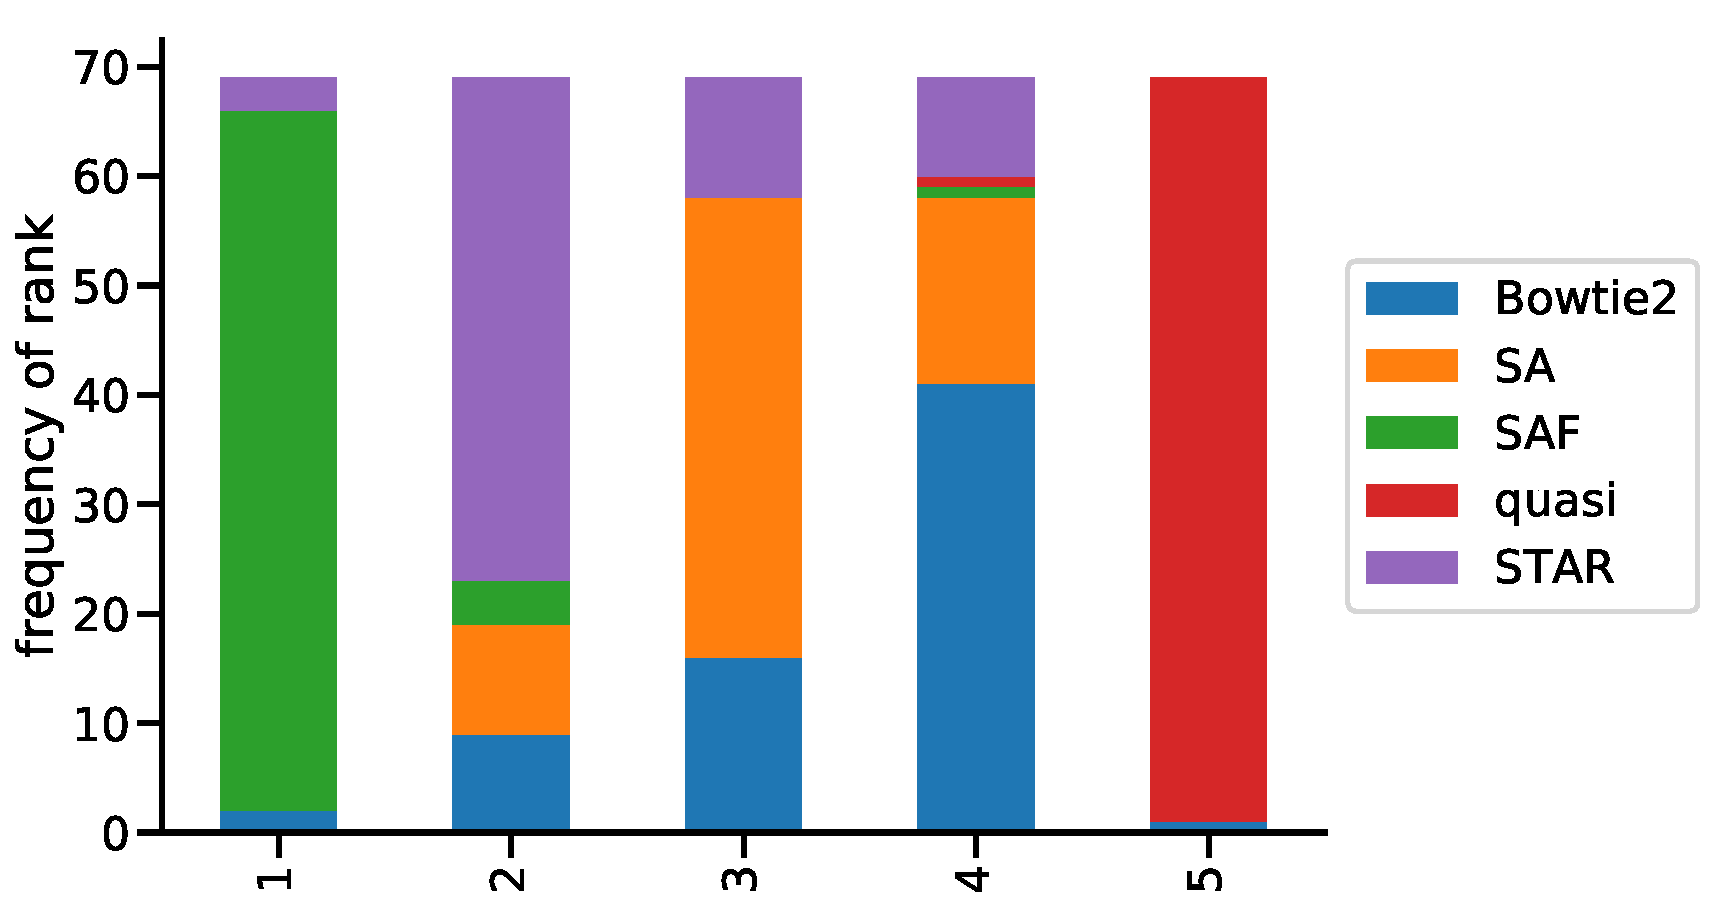
\includegraphics[width=\linewidth]{selal/bulk_ranks.pdf}
	    \caption{}
	    \label{fig:bulk_ranks}
    \end{subfigure}
    ~
    \begin{subfigure}[t]{0.45\textwidth}
        \centering
	    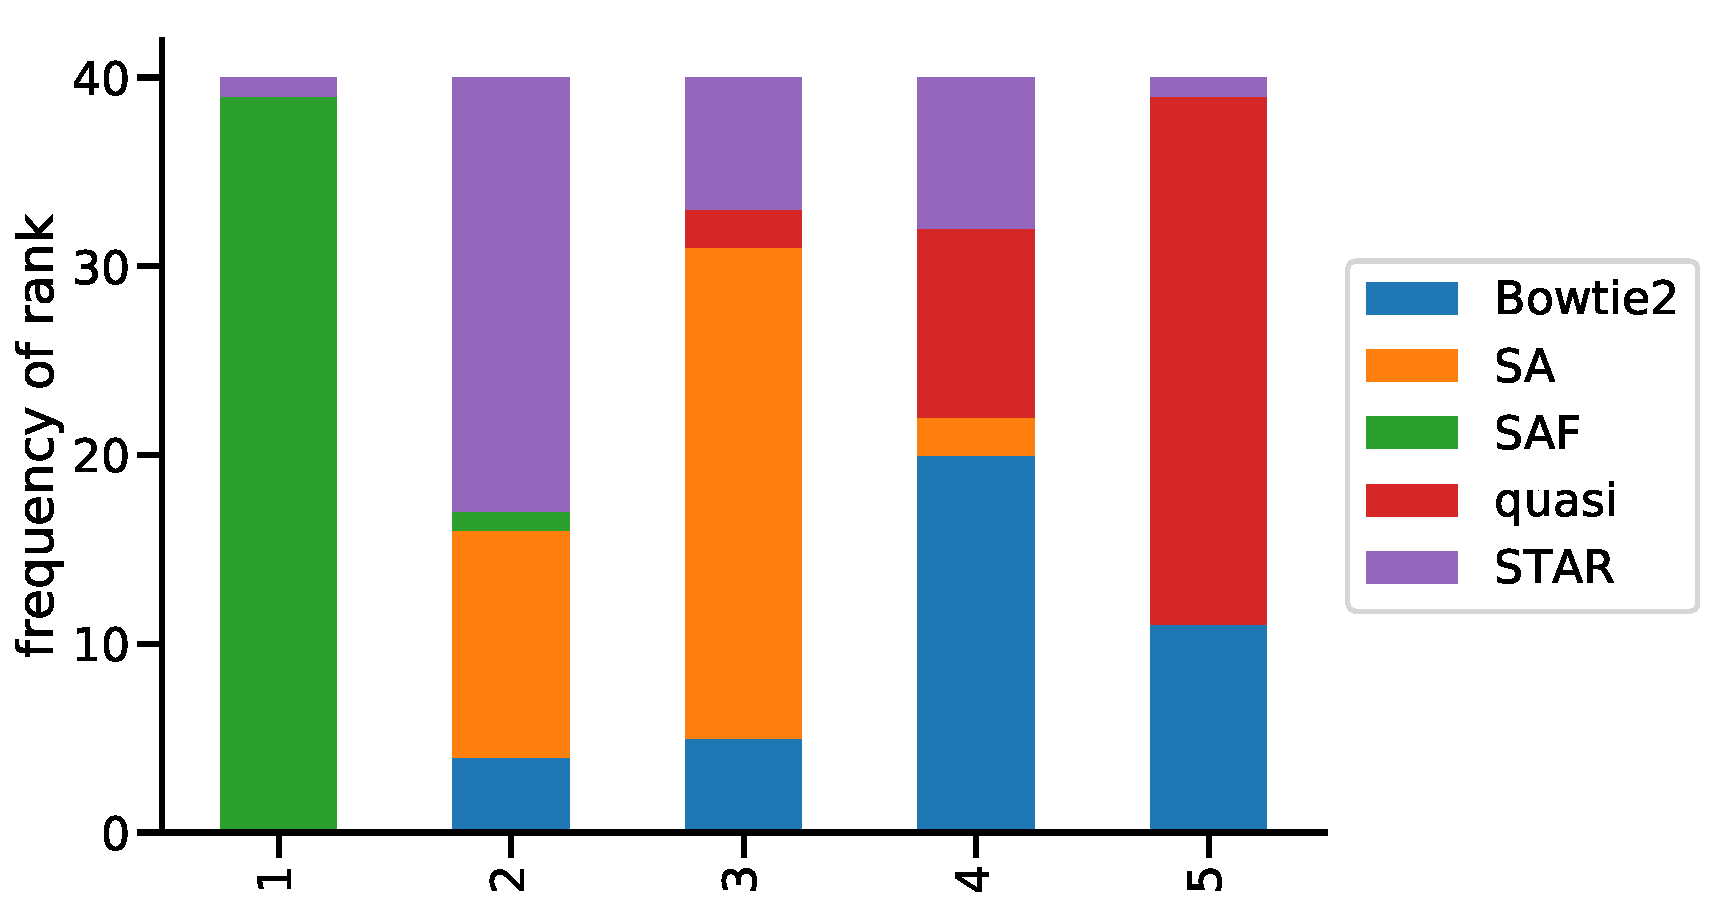
\includegraphics[width=\linewidth]{selal/sc_ranks.pdf}
	    \caption{}
	    \label{fig:sc_ranks}
    \end{subfigure}
     \caption{\textbf{Rank of each method in terms of correlation with oracle.} Histogram of the ranks across the $69$ bulk samples (a) and 
       the $40$ full-length single-cell samples (b), of different
       methods in terms of the Spearman correlation of the method's abundance with
       the oracle. Here, the most correlated method is assigned rank 1, while
       the least correlated method is assigned rank 5.}
    \label{fig:rank}
\end{figure}

In terms of Spearman correlation between all methods, we observed the
  highest average pairwise concordance between the oracle and \saf, 
  in both the bulk and single-cell samples (\Cref{fig:swarm}).
  \saf had the highest rank in order of its correlation with the
  oracle across the bulk and single-cell samples (histogram of the
  frequencies of these ranks in \Cref{fig:rank}), and had the closest
  mapping rate compared to the oracle (\Cref{fig:mrate}).
  Among the alignment-based methods, 
  STAR displayed higher correlation with the oracle --- especially in full-length single-cell
  samples --- than did Bowtie2; a reversal of the trend that was observed 
  with respect to the ground truth on the simulated data in~\Cref{subsec:initial_sim,subsec:variant_sim}.
  Further, the overall correlations were lower, and the differences were larger, in the full-length
  single-cell samples than in the bulk samples.  Bowtie2 tended to correlate highly with \hsa, while
  STAR tended to correlate highly with \saf, though \hsa and \saf were, themselves, highly correlated.
  Also, Bowtie2 and STAR both had a higher correlation with the oracle than they did with each other.
  This was somewhat expected since the oracle was created by considering the alignments of both Bowtie2 and 
  STAR.  However, this also suggested that the manners in which these approaches diverged from the oracle 
  were largely distinct (i.e. they made different types of mistakes in alignment).
  The quantifications from lightweight mapping exhibited the lowest overall correlation with the oracle. 
  These results were also indicative of the types of divergence between simulated and
  experimental datasets that we expected to observe. The trend was similar when
  comparing TPM values after discarding transcripts shorter than $300$bp
  (\Cref{tab:withoutshortsc,tab:withoutshortbulk}) and when comparing read counts predicted by each
  method, instead of TPM, as shown in~\Cref{fig:swarmcount}. For the
    purpose of analyzing the performance of a lightweight mapping algorithm
    other than \qm, we also compared the estimates from
    \kallisto~\citep{kallisto} against the other methods on these $109$
    experimental datasets. It displayed the lowest overall correlations with the
    alignment-based approaches (\Cref{fig:kallisto}). This may be due, in part,
    to the fact that it altered both the quantification and mapping methodology,
    and because there were no options to control for structural constraints on
    the reported mappings (i.e.\@ orphaned and dovetailed mappings). Thus, for
    consistency, we excluded it from the other analyses in the
    manuscript.

Finally, while one would not typically regard any of the
  average correlations in~\Cref{fig:swarm} as poor, it is important to properly
  frame these differences as representing the aggregate Spearman correlation,
  across the samples, each quantifying $206,694$ transcripts (wherein most
  features are properly quantified as having an abundance of $0$). A correlation
  coefficient is a single coarse metric, and as demonstrated
  in~\Cref{subsec:variant_sim}, even substantial quantification differences
  across thousands of transcripts can nevertheless result in small differences
  in the summary correlation. To explore some of the transcripts with large differences
  in quantification across methods, we performed differential transcript
  expression analysis across methods on the $109$ samples, using
  limma-trend~\citep{law2014voom}. The counts per million (CPM) for the top 100,
  500, and 1000 transcripts is shown in~\Cref{fig:heatmap}. This highlighted the
  divergence of the methods from each other, in terms of quantification and
  revealed clusters of transcripts that were differentially expressed under each
  method. Further, as described in~\Cref{sec:DE}, such differences can lead to
  considerable changes in which genes are found to be differentially
  expressed.
  

\subsection{Simulation fails to capture complex patterns of real experiments, even when seeded from experimental abundances}
\label{subsec:sim_from_real}

In principle, if the specific transcript expression
profile was the primary source of quantification difficulty among the different approaches, we
should be able to reproduce the types of divergence we observed between
different methods in the experimental data
(i.e.~\Cref{fig:swarm}) in simulation by simply creating
simulations where the transcript expression profile is seeded with the estimated
abundance results obtained from the experimental samples (using e.g.\@ the
Bowtie2-derived quantifications).
To test this hypothesis, we used Polyester~\citep{polyester} to simulate 109
synthetic experiments where the expression profiles in each simulated sample
were matched to those of the corresponding experimental sample's transcript
abundances generated by the Bowtie2-based pipeline. 

\begin{figure}[t!]
    \centering
     \begin{subfigure}[t]{0.7\textwidth}
     \centering
  	  	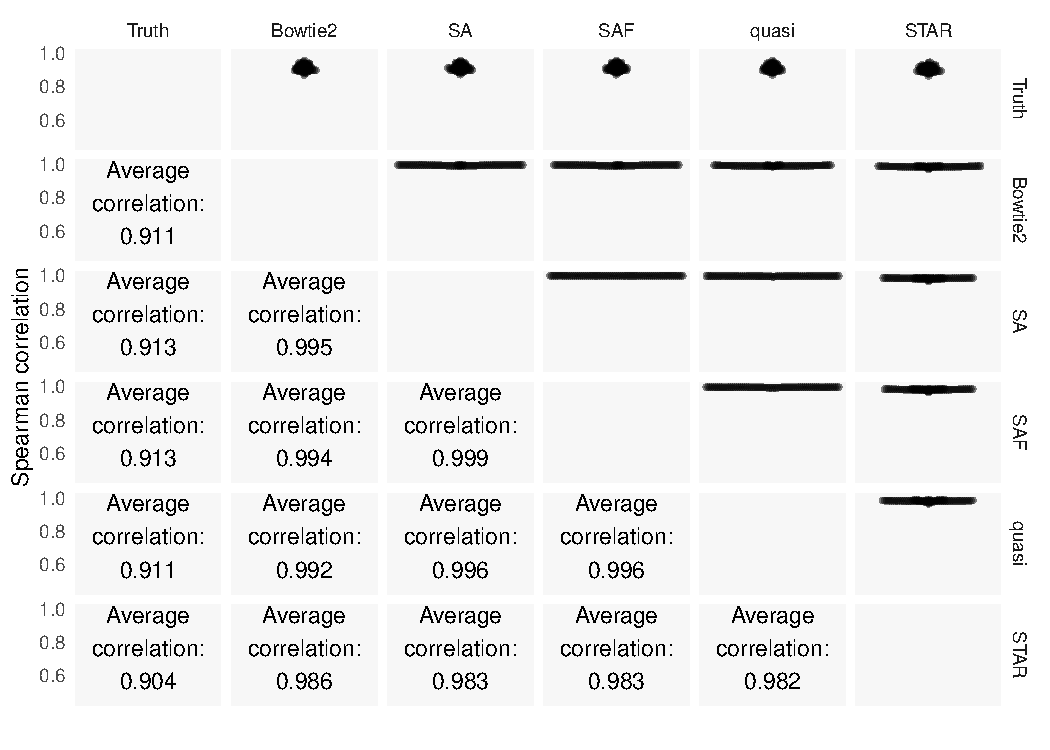
\includegraphics[width=\linewidth]{selal/bulk_pairwise_correlations_sim_data.pdf}
		\caption{Bulk}
    \end{subfigure}
     \begin{subfigure}[t]{0.7\textwidth}
     \centering
  	  	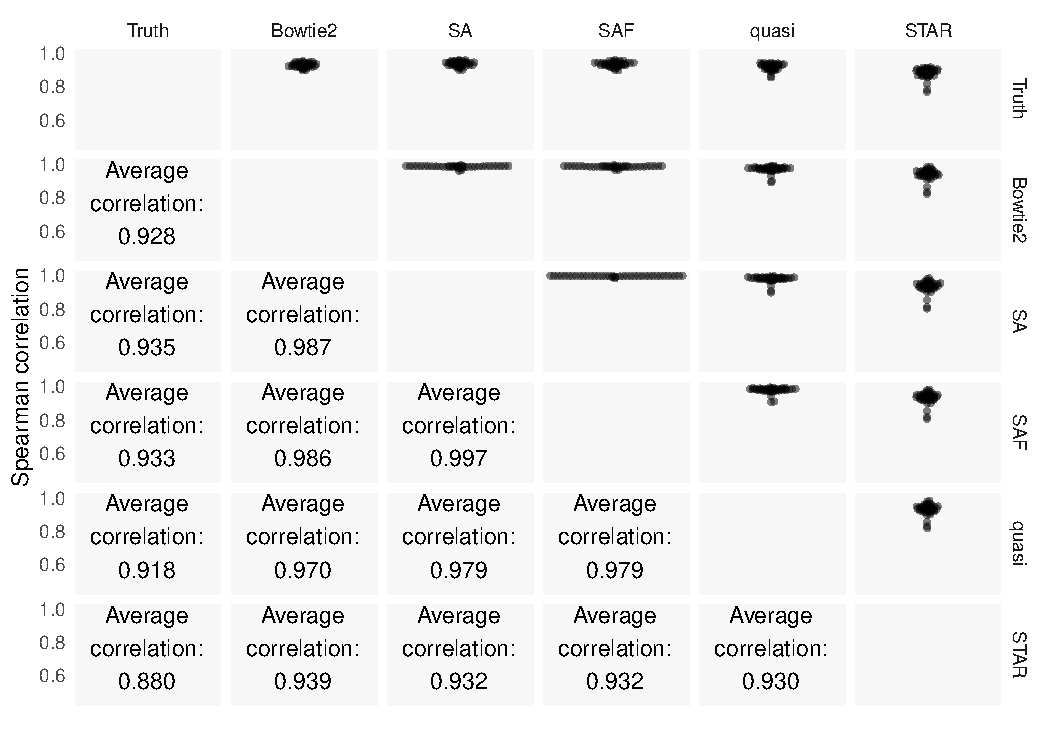
\includegraphics[width=\linewidth]{selal/singlecell_pairwise_correlations_sim_data.pdf}
		\caption{Single-cell}
    \end{subfigure}
    \caption{\textbf{Performance of each method on bulk datasets simulated using Polyester.}
    The top half of the matrix shows swarm plots of pairwise correlations of counts predicted by the different approaches with each
      other and with the true read counts on the simulated samples generated
      using the experimentally-derived abundances from Bowtie2 and \salmon. The bottom half shows the
      average Spearman correlations between the different methods across the
      $109$ simulated datasets.}
     \label{fig:swarmsim}
\end{figure}

We quantified transcript abundance in all of
these simulated samples using the same methods we considered in the experimental
data. For transcript counts from simulated data, the correlation
with the truth, and between methods, is shown in~\Cref{fig:swarmsim}. Shown in~\Cref{fig:swarmsimTPM} is
the correlation values calculated using the predicted TPMs instead of read counts. Clearly, the correlations among
methods was markedly higher in the simulated data than in the experimental data (\Cref{fig:swarm}),
and multiple methods even showed a correlation $\ge 0.99$. The variability between
the samples was also considerably lower than what we observed in experimental
data. This further suggested that comparison of correlations on simulated data is
likely to be only a starting point in assessing different methods, as many
salient differences that arise in experimental data disappear when the
comparisons are performed on simulated data.

The variation in correlation across the simulated samples was inconsistent 
with the hypothesis that the distribution of
transcript expressions alone is sufficient to simulate quantification scenarios
as complicated as those observed in experimental data. This suggests that there
are important aspects, apart from the underlying transcript expression profiles
and simulation of read errors, that the simulation failed to capture. Though
we do not know all such features, some important biological features, like
structural variations (SV), SNP variants and small indel variants, which are
sample-dependent rather than reference-dependent, are missing. 
  Furthermore, transcription and sequencing in experimental RNA-seq samples are
  not limited to the fully-spliced, annotated transcript sequences present in a
  reference database, even for organisms as well-characterized as human and
  mouse. Reads derived from unannotated genomic regions that bear resemblance to
  annotated transcripts, or which only partially overlap the annotated features,
  can then be spuriously aligned to the annotated features, leading to
  inaccurate quantification of their abundances. Since such effects can vary from sample-to-sample,
  they do not affect the estimated expression of the annotated features in a uniform way, and can
  therefore affect subsequent analyses, such as differential expression testing.

We realize that sample-dependent features are difficult to simulate, and that all
of the major features or processes affecting a sample may not even be known, but
not including such effects diminishes the realism of the simulated data, and
this lack of complexity can be observed in the divergence of the performance of
different quantification pipelines compared to how they performed in experimental
samples. Identifying other factors present in experimental datasets but lacking
in simulations, and determining how to faithfully simulate these factors, seems
an important area for future research. 

\subsection{Quantification differences can affect differential gene expression analysis}
\label{sec:DE}
\begin{figure}[ht!]
    \centering
    \begin{subfigure}[t]{0.49\textwidth}
        \centering
  	  	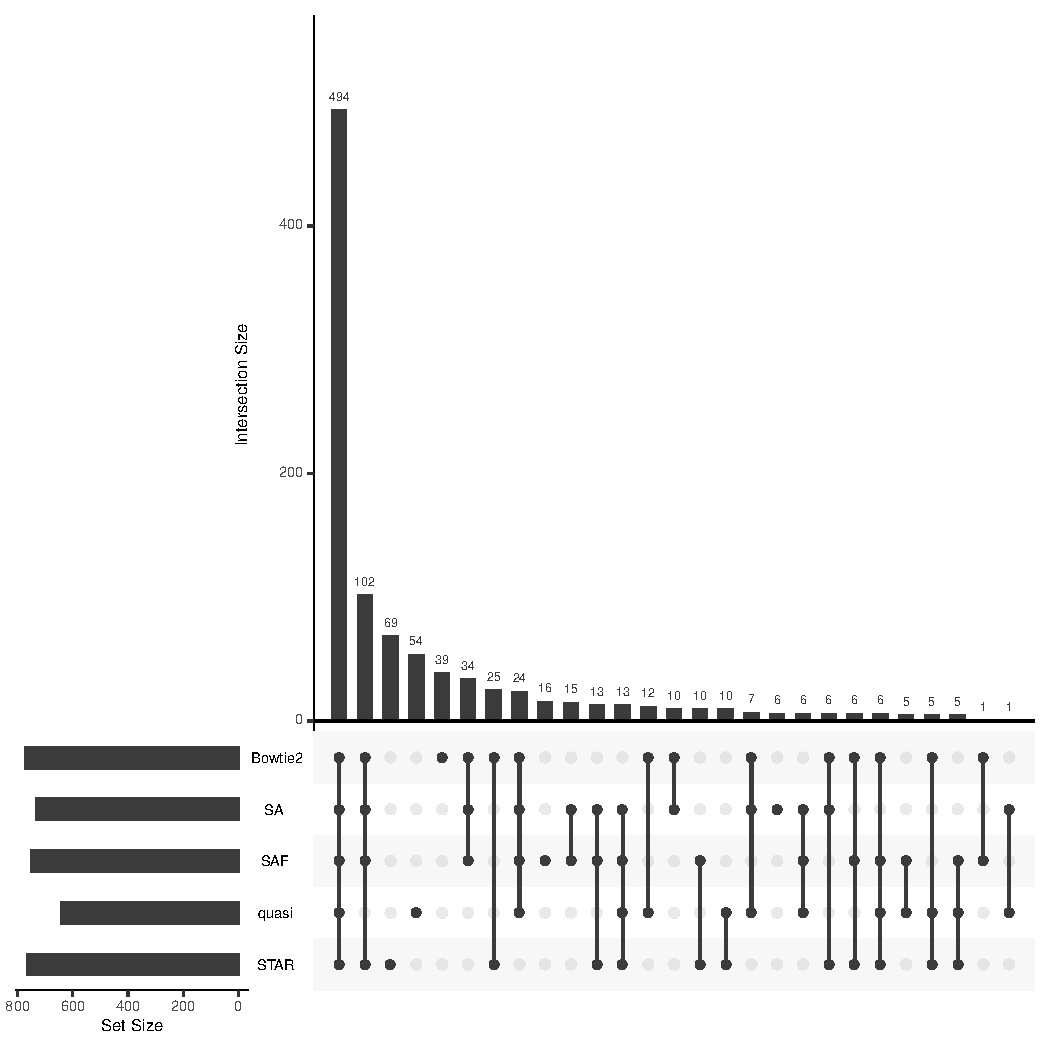
\includegraphics[width=\linewidth]{selal/de_als.pdf}
		\caption{}
    \end{subfigure}
    ~ 
    \begin{subfigure}[t]{0.49\textwidth}
        \centering
  	  	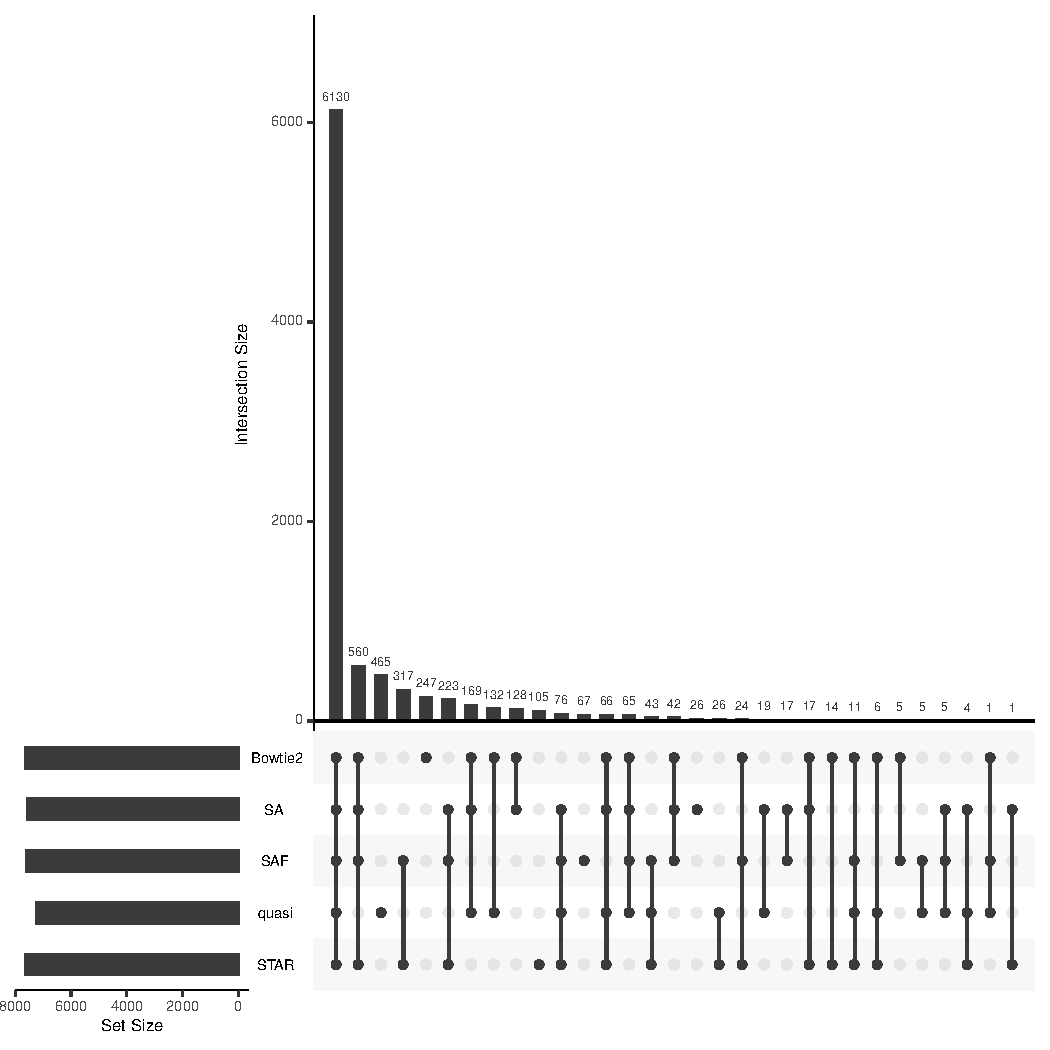
\includegraphics[width=\linewidth]{selal/de_hsv.pdf}
		\caption{}
    \end{subfigure}
    \caption{\textbf{Differentially expressed genes predicted using each method in $2$ datasets.} 
    Comparison of sets of differentially expressed genes, and their overlaps, computed using each method.
    The analysis was done on $2$ datasets containing multiple replicates of control and infected samples, from human ALS
    motor neurons (a) and HSV-1 infected cells (b). In each plot, the combination matrix at the bottom shows the intersections between the sets and the bar above
      it encodes the size of the intersection. }
    \label{fig:dge}
\end{figure}

One of the most common downstream uses of transcript and gene abundance estimates is
differential gene expression analysis. Errors in the
transcript quantification phase can lead to incorrect detection of
differentially expressed genes across conditions. Therefore, quantification
is a crucial step for accurate differential gene expression (DGE) estimation and
other downstream analyses. To show the influence of quantification on DGE, we
performed a case study on two recently published datasets, where sequencing was
done for RNA profiling of differences between the healthy and diseased samples. 
The first dataset is comprised of human ALS motor neurons and studies the effect 
of the SOD1A4V mutation (2 patient-derived samples) versus (3) isogenic controls (PRJNA236453~\citep{kiskinis2014pathways}). The
second dataset contained $3$ replicates each of uninfected and herpesvirus (HSV-1) infected 
samples (PRJNA406943~\citep{shi2018deep}). Hence, the design of this study will highlight how
misquantifications, possibly arising from incorrect alignments, can impact DGE analysis.


We aligned and quantified reads from all samples using the \hsa, \saf, \qm, STAR and
Bowtie2 pipelines. The transcript-level counts were summed to the gene level
using tximport~\citep{soneson2015differential} and differential expression analysis was
performed using DESeq2~\citep{love2014moderated}. Genes were called as
differentially expressed between the conditions, for each tool, if they had an adjusted p-value
$\leq 0.01$ (i.e. an FDR (false discovery rate) of $0.01$ was used).  The overlaps of the
resulting gene sets were computed. While we had focused on transcript-level
analysis in the paper until now, here we looked at differences in gene-level
differential expression. This demonstrated that the quantification issues caused
by lightweight mapping or misalignment of reads could be of relevance even when
one is performing gene-level analyses.

The results, visualized using UpSetR~\citep{conway2017upsetr} and presented
  in~\Cref{fig:dge}, show that lightweight mapping tended to miss the largest number 
  of genes discovered as DE by all other approaches (i.e. the second-largest set in 
  both examples, after the consensus set containing genes found by all approaches, was
  the set of genes found by all approaches except for lightweight mapping). The mean
  adjusted p-value of these genes under \qm was $0.034$ and $0.069$ in the two datasets,
  showing that lightweight mapping tended to deviate by a large margin from the other methods. Further,
  lightweight mapping also tended to discover a considerable number of distinct genes 
  that were called as differentially expressed by this approach but not by any of the other approaches
  (alignment-based or selective-alignment-based), and which may have represented false positives.
  In each sample, the number of genes with at least one transcript shorter than
  $300$bp constituted less than $10\%$ of the total number of genes called
  differentially expressed only under the lightweight mapping based
  quantification, so this effect was unlikely to be driving these differences.
  In all cases, despite having a large overlap
  in DE calls with the alignment-based methods, \hsa produced quantifications that yielded
  the fewest isolated DE calls. A similar trend was observed when using an FDR of $0.05$, as shown in~\Cref{fig:suppdge}(a,b)
  and when including \kallisto as a lightweight mapping method as well, as in~\Cref{fig:suppdge}(c,d). 
  These results suggested that, when
  the sequenced reads tend to vary more from the reference, as might be the case
  in many diseased cells, lightweight mapping methods can lead to
  misquantifications that can eventually lead to false positives and false
  negatives in downstream differential gene expression studies.
 
\subsection{Quantification differences can affect differential transcript expression analysis}
\label{sec:DTE}

\begin{figure}[ht!]
	\centering
	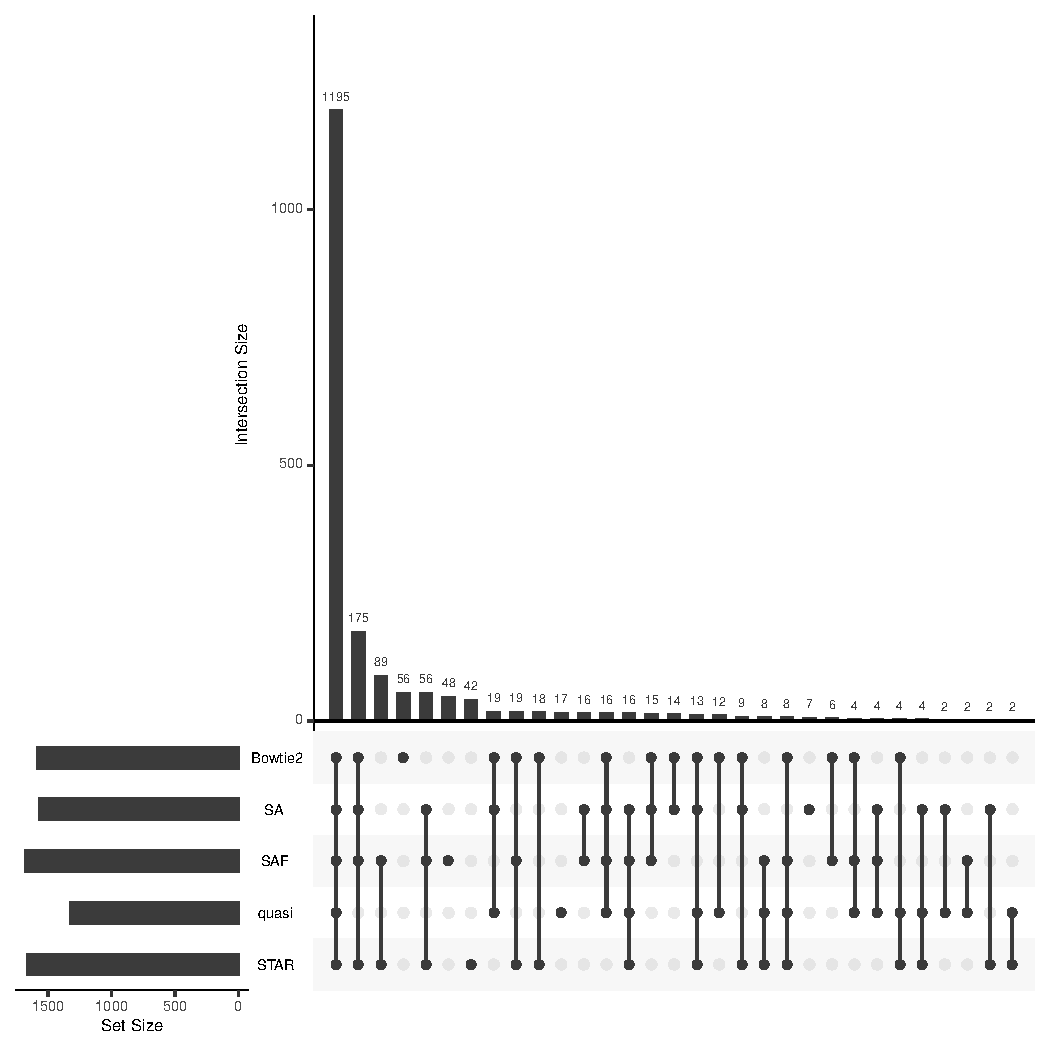
\includegraphics[width=0.5\linewidth]{selal/de_zika.pdf}
    \caption{\textbf{Differentially expressed transcripts predicted using each method.} 
    Comparison of sets of differentially expressed transcripts, and their overlaps, computed using each method.
    The analysis was done on a dataset containing multiple replicates of control and zika infected samples.
 	In each plot, the combination matrix at the bottom shows the intersections between the sets and the bar above
      it encodes the size of the intersection.}
    \label{fig:dte}
\end{figure}

Errors in quantification can impact differential expression analysis not just at the gene level, 
but at the transcript level as well. To show this impact, we selected a dataset that has recently been 
used to study the impact of the zika virus on the transcriptome in human neural progenitor cells (PRJNA313294~\citep{tang2016zika}). 
Note that, for consistency, we have used the same design as previous analyses and included both the
paired-end and single-end datasets. Hence, there are $2$ control and $2$ infected samples under
each protocol. As with the gene level analysis, the alignment and quantification for all samples was done using the \hsa, \saf, \qm, 
STAR and Bowtie2 pipelines. Transcript differential expression analysis was done using sleuth~\citep{pimentel2017differential} and 
transcripts were called as differentially expressed at an FDR of $0.01$. 

The results are presented in~\Cref{fig:dte} and
show, as with the gene level analysis, that lightweight mapping tended to be the biggest outlier in terms of 
missing transcripts called as DE under all other methods.  Here, we also observed a considerable 
set of transcripts (89) discovered only by \saf and STAR, and not by any other approach. 
For transcripts called as differentially expressed by the other methods but 
missed by \qm, the mean adjusted p-value was $0.027$. At an FDR of $0.05$, this increased to 
$0.09$, highlighting the difference between the quantification estimates from lightweight mapping
and alignment-based methods (results visualized in~\Cref{fig:suppdte}(a)). The results presented 
in~\Cref{fig:suppdte}(b) show the distribution of the DE transcripts if we included \kallisto as a
mapping and quantification method in this analysis. As before, the lightweight mapping methods, \qm and
\kallisto, tended to deviate from the alignment based methods. We also abserved that the number of DE transcripts
are the lowest under these methods. 

\section{Discussion \& Conclusion}
\label{sec:conclusion}

We compared and benchmarked the effects of using different alignment and mapping
strategies for RNA-seq quantification, and discussed the caveats implied by
different approaches. We observed that methods that perform traditional alignment
of the reads against the transcriptome can produce results that are sometimes
markedly different from the results produced by lightweight mapping methods. We
also observed that performing spliced alignment to the genome and then projecting
these alignments to transcriptome can also produce divergent results compared
to directly aligning to the transcriptome.


At the same time, we proposed and benchmarked a new hybrid alignment method, \hsa,
which provides an efficient alternative to lightweight mapping that produces
results much closer to what is obtained by performing traditional alignment.
This approach overcomes the shortcomings of lightweight mapping both in terms of
sensitivity and specificity, as it is able to determine appropriate alignments
when lightweight approaches return either suboptimal mappings or no mapping, and
it is also able to better distinguish the optimal alignment loci among a set of
otherwise similar sequences. Some key differences that lead to the improved
accuracy of SA are an increase in mapping sensitivity (i.e.\@ more initial
mapping loci are explored), a more comprehensive and systematic mechanism for
scoring potential mapping loci (making use of the match chaining algorithm
of~\citet{minimap2}), and an actual alignment scoring phase that provides
precise information about the quality of each retained mapping, allowing
filtering out of spurious mappings that should not be reported. Moreover, the
\hsa approach can take as input a set of decoy sequences, enabling it to avoid some of the
spurious transcriptome mappings reported by Bowtie2, when, in reality, the read
aligns better to an unannotated genomic locus than to the annotated
transcriptome.

The results of benchmarking the different approaches on multiple simulated and
experimental datasets lead to a number of conclusions. First, despite the fact
that major strides have been made in improving the realism of simulated RNA-seq
data, there still remain numerous ways in which simulated data fail to
recapitulate the intricacies and challenges of experimental data. One of these
is the fact that simulations are almost always carried out on precisely the same
transcriptome that is used for quantification, while, in experimental samples,
individual variation exists between the sample being assayed and the
transcriptome being used for quantification. Another effect not
  commonly captured in simulation, but prevalent in real data, is the sequencing
  of reads from unannotated, alternatively-spliced transcripts, from transcripts
  with retained introns, from otherwise unannotated genomic loci sharing
  sequence-similarity with annotated transcripts, and from contamination with the 
  sample that may share sequence similarity, to some extent, with the target transcriptome. 
  These effects, along with others that we have not fully characterized in this manuscript, make alignment
  and quantification in experimental samples much more challenging than in
  simulated data. Hence, we observed that when quantifying across a broad sample
of experimental datasets, the quantification results obtained using different
mapping and alignment approaches can demonstrate considerable variation.
Together, these results suggest that quantification based purely on lightweight
mapping approaches can fail to achieve the accuracy that is obtainable by the
same inference algorithms when using traditional alignments, and that these
errors in quantification can also affect downstream analyses, even at the gene
level (as discussed in~\Cref{sec:DE}). It also suggests that there is practical
room for improvement, even in the most accurate existing alignment approaches, at least
for the purpose of quantifying the abundance of annotated transcripts.

While it has been previously
reported~\citep{direct_comparison} that pseudoalignment to the transcriptome
results in comparable quantification accuracy to alignment to the genome, the analyses
performed in this manuscript suggest that alignment to the transcriptome,
lightweight mapping to the transcriptome, and alignment to the genome yield
quantification results that are sometimes markedly different.
%do not support that conclusion.
There are a few reasons that the analyses carried out in this paper lead to a
different conclusion on this question. First, the focus here is much more on
experimental as opposed to simulated data. While we found that differences
between lightweight mapping and alignment do exist in simulation, the magnitude
of their effect on quantification is generally much smaller than is observed in
experimental data. Second, while lightweight mapping to the transcriptome and alignment
to the genome do yield different quantification results, we also considered
traditional alignment to the
transcriptome, expanding upon the different common approaches that are taken
when aligning reads prior to transcript quantification. Finally, \citeauthor{direct_comparison}~\citep{direct_comparison} 
preprocess both alignments and
pseudoalignments into equivalence-class counts (the count of fragments deemed
compatible with different subsets of transcripts). Then, from these reduced
statistics, abundance estimation is performed. This transformation 
discards factors that contribute to conditional fragment assignment
probabilities like alignment scores (where applicable), fragment lengths, fragment positions, etc.
In the analysis presented here, we accounted for such conditional fragment
probabilities in the online phase of transcript quantification, and incorporated
them (approximately) into the sufficient statistics via the use of
range-factorized equivalence classes~\citep{ddfact}. Discarding such conditional
probabilities could potentially diminish true differences that exist in the
underlying mappings that may, depending on the complexity of the quantification
model, have an effect on quantification estimates. All of these factors may
account for the sometimes considerable differences in quantification accuracy
observed downstream of different lightweight mapping and alignment procedures.
While we focused on quantification and differential expression,
the observations made in this manuscript about the sensitivity
  and accuracy of different alignment approaches may extend to other
downstream analyses as well, such as trans-acting expression quantitative trait
locus (eQTL) detection \citep{saha2018false}.

Considering only the results on simulated data, one
  might prefer quantification based on alignment or lightweight mapping of
  sequencing reads directly to the transcriptome, rather than performing
  alignment to the genome followed by projection to the transcriptome. One
  would also observe only small differences between lightweight mapping and
  alignment to the transcriptome. However, our analyses in experimental
  data suggested that the increased complexity in real RNA-seq experiments
  leads to more divergent behavior.  In both the bulk and full-length single-cell samples analyzed, \saf yielded
  the highest overall correlation with the oracle, despite the fact that the oracle 
  is derived from a combination of the Bowtie2 and STAR alignment results. 
  Among the methods based on traditional
  alignment, alignment to the genome (using STAR, and projecting the
  resulting alignments to the transcriptome), seemed to display the best
  concordance, on average, with the quantifications resulting from oracle
  alignments. \hsa yielded similar but slightly better accuracy than alignment
  to the transcriptome using Bowtie2.  This is likely, in part, because it is accounting for the 
  sequence-similar decoys that can lead alignment to only the target transcriptome 
  astray. The main benefit of \saf is that it aligns to a reference index that contains both the fully-spliced
  transcript sequences as well as the entire underlying genome (as potential decoy sequence).
  This allows \saf to obtain the type of sensitivity that is exhibited by approaches like 
  Bowtie2 and \hsa when the read truly arises from the annotated
  transcriptome, but also allows it, like STAR, to avoid spuriously aligning
  a read to an annotated transcript when it is better explained by some other
  genomic locus. In the experimental data, both alignment-based approaches
  and selective-alignment methodologies performed better than
  \qm, though the manner in which these methods differ from \qm, and from 
  each other, were not identical.

When trying to choose an approach, a choice can be made by the user
performing the analysis based on any time-accuracy tradeoff they wish to
make. In terms of speed, we observed that \qm is the fastest approach,
followed by \hsa and \saf and then STAR. Bowtie2 was considerably slower than
all three of these approaches. However, in terms of accuracy, we found that
\saf yielded the best results, followed by alignment to the genome
(with subsequent transcriptomic projection) using STAR and \hsa (using
carefully selected decoy sequences). Bowtie2 generally performed similarly to
\hsa, but without the benefit of decoy sequences, seemed to admit more
spurious mappings. Finally, lightweight mapping of sequencing reads to the
transcriptome showed the lowest overall consistency with quantifications
derived from the oracle alignments. The analyses carried out in this
manuscript suggest that, with respect to accurate quantification of annotated
transcripts, alignment scoring is an important component, but the various
pre-existing alignment approaches excelled in different cases. \hsa takes
steps toward addressing the shortcomings of existing alignment based
approaches without making large compromises on speed. This is done by
indexing parts of the genome that are sequence-similar to the transcriptome or,
as in the case of \saf, the entire genome in addition to the annotated transcriptome, hence
exhibiting the sensitivity of Bowtie2 in transcriptomic alignment, while
avoiding the spurious alignment of reads that do not truly originate from
some annotated transcript, like STAR. This approach seemed to provide the
highest overall accuracy, at least for the purposes of quantifying an
annotated set of transcripts.